\documentclass[a4paper]{exam}
\usepackage[utf8]{inputenc}
\printanswers\usepackage[utf8]{inputenc}
\usepackage[top=2in, bottom=1.25in, left=1.25in, right=1.25in]{geometry}
\usepackage{graphicx}
\usepackage{url}
\usepackage{subcaption}
\usepackage{amsmath, amsthm, amssymb}
\usepackage{epstopdf}
\usepackage{csquotes}
\usepackage{tikz}
\usepackage{placeins}
\usepackage{hyperref}
\usepackage{tikz,pgfplots}
\usepackage{listings}
\usepackage{mwe}
\usepackage{systeme}
\usepackage{cleveref}
\usepackage{qtree}

\usepackage{color}


\definecolor{codegreen}{rgb}{0,0.6,0}
\definecolor{codegray}{rgb}{0.5,0.5,0.5}
\definecolor{codepurple}{rgb}{0.58,0,0.82}
\definecolor{backcolour}{rgb}{0.95,0.95,0.92}

\lstdefinestyle{mystyle}{
    backgroundcolor=\color{backcolour},
    commentstyle=\color{codegreen},
    keywordstyle=\color{magenta},
    numberstyle=\tiny\color{codegray},
    stringstyle=\color{codepurple},
    basicstyle=\footnotesize,
    breakatwhitespace=false,
    breaklines=true,
    captionpos=b,
    keepspaces=true,
    numbers=left,
    numbersep=5pt,
    showspaces=false,
    showstringspaces=false,
    showtabs=false,
    tabsize=2
}

\lstset{style=mystyle}


\title{Homework 2 - Parallel Programming for Large Scale Problems - SF2568}
\author{Gabriel Carrizo}
\date{December 2017}

%-------------------------------------------------------
\begin{document}

\maketitle

\pagebreak
\begin{questions}

\section{Broadcast Operation}

\addpoints\question Design an algorithm for the broadcast operation only using point-to-point comunication.

\begin{solution}
The brodcast operation is an operation that sends the information of one node to all other processes. Using recursive doubling one can `spread' amongst processes, much like an infection moves through a host.

The idea is that the process with the data sends its data to another process. Once that process also possesses the data, both processes send the data to two other processes. Now we have four processes with data and all four can send data to four other processes. This procedure repeats until all processes posses the data (see figure \ref{graph}).

The complexity of the solution in parallel is dependent on the number of processors used.

See Listing \ref{lst:label} for pseudoecode. (Made under the assumption that $P=2^D$)
\end{solution}

\begin{figure}
  \center
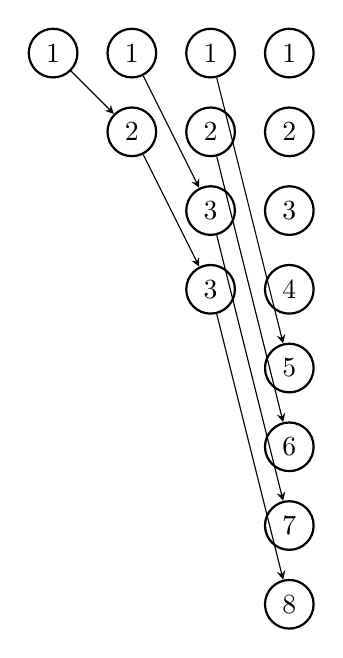
\begin{tikzpicture}
  \begin{scope}[every node/.style={circle,thick,draw}]
      \node (10) at (0,5) {1};

      \node (11) at (1,5) {1};
      \node (21) at (1,4) {2};

      \node (12) at (2,5) {1};
      \node (22) at (2,4) {2};
      \node (32) at (2,3) {3};
      \node (42) at (2,2) {3};

      \node (13) at (3,5) {1};
      \node (23) at (3,4) {2};
      \node (33) at (3,3) {3};
      \node (43) at (3,2) {4};
      \node (53) at (3,1) {5};
      \node (63) at (3,0) {6};
      \node (73) at (3,-1) {7};
      \node (83) at (3,-2) {8};
  \end{scope}

  \tikzset{thin arc/.style={->, black, fill=none, thin, >=stealth, text=black}}

  \draw[thin arc] (10) -- (21);

  \draw[thin arc] (11) -- (32);
  \draw[thin arc] (21) -- (42);

  \draw[thin arc] (12) -- (53);
  \draw[thin arc] (22) -- (63);
  \draw[thin arc] (32) -- (73);
  \draw[thin arc] (42) -- (83);

\end{tikzpicture}
\caption{Graph representation of broadcasting with recursive doubling.}
\label{graph}
\end{figure}


\lstinputlisting[caption={Pseudocode for broadcasting operation.},label={lst:label},language=Python]{broadcast.py}


\addpoints \question Do a (time-)performance analysis for your algorithm.

\begin{solution}
  blabla
\end{solution}

\addpoints \question How can the scatter operation be implemented using $O(log P)$ communication steps?

\begin{solution}
Assuming we know the length $N$ of the data and that $N=2^K$, where $K\geq P$, such that the data is evenly distributed among the processes.
\end{solution}

\section{Transpose}
\begin{solution}
  Assuming that what the algorithm from class leaves us with a grid with load balanced data distribution where each process has address $P[row,col]$:

  \begin{equation*}
    M =
    \begin{bmatrix}
      y_0 & y_0 & ... & y_0 \\
      y_1 & y_1 & ... & y_1 \\
      ... & ... & ... & ... \\
      y_P & y_P & ... & y_P
    \end{bmatrix}
  \end{equation*}

  Which we want to transpoe into:

\begin{equation*} M^T =
  \begin{bmatrix}
    y_0 & y_1 & ... &y_P\\
    y_0 & y_1 & ... &y_P\\
    ... & ... & ... &...\\
    y_0 & y_1 & ... &y_P
  \end{bmatrix}
\end{equation*}

We observe that the diagonal of the matrix $M$ holds values that should be broadcast to the entire column.

There are two approaches that work with the broadcast algorithm suggested in the previous section.

The first one is to send the data from the first column to the first row, such that P[0,1] sends to P[1,0], P[0,2] send to P[2,0], etc. Once the first row is filled with its initial value the broadcast be performed, just like in the previous section but for each column individually.

The second approach I will suggest is to perform a cyclic shift for the rows of each column s.t. every diagonal element is shifted to the the first row of matrix M. This method requires some adjustments so the processes send and recieve to and from the correct index (see Listing \ref{lst:transpose})

The first approach requires an extra communication step and will also require sending data to some processes on the diagonal that already posses the data. The second approach requires some extra calculation steps but should overall be quicker since it requires fewer communication steps.
\end{solution}

\lstinputlisting[caption={Pseudocode for transpose with the broadcast operation operation.},label={lst:transpose},language=Python]{transpose.py}



\end{questions}
\end{document}
